\documentclass[conference]{IEEEtran} % Usa la classe IEEEtran per formattazione simile

\usepackage{amsmath}
\usepackage{graphicx}

\begin{document}
\bstctlcite{IEEEexample:BSTcontrol}

\title{Exploring the Adversarial Robustness of AI-generated Image Detectors}

\author{
    \IEEEauthorblockN{Thomas Lazzerini, Samuele Cappelletti, Martina D'Angelo}
    \IEEEauthorblockA{
        University of Trento
    }
}

\maketitle

\begin{abstract}
    Nowadays, there exists many image generators, so it is important to discriminate between synthetic images and real ones. In this regard, many detectors has been proposed but, at the same time, also many attacks to this detectors has been developed to interfere with their detection capabilities. In this report we present a general overview about some detection techniques and some recently developed attack techniques. 
\end{abstract}

\section{Introduction}
    Synthetic images are now flooding the real world, from online dating sites to social media, fake profiles and scams are everywhere. While some images are funny and harmless, others could be exploited by malicious users \cite{carlini2020evading}. In relation to this, in the image forensic field there is a continuous fight between \textit{image detectors} and \textit{adversarial attacks}. On one hand, the detectors try to discriminate synthetic images from real ones, while, on the other hand, the attacks try to trick the detectors by manipulating the images, both real and synthetic. In order to detect synthetic images, we have two main types of techniques: the \textit{high-level forensic techniques} and the \textit{low-level forensic techniques}. The former focuses on physical inconsistencies \cite{farid2022lighting}\cite{farid2022perspective} and on repeated and uniform patterns \cite{mundra2023exposing}, both of which are mostly visible to the human eye. While, the latter focuses on pixel-level artifacts, almost invisible to the human eye. Since image generators are becoming smarter every day and are able to avoid generating high-level artifacts, we prefer to rely on the low-level ones.

\section{Detectors}
    In this section we provide an overview about some detection techniques. In particular, a smart use of \textit{CLIP} to extract the feature vectors from the images \cite{cozzolino2024raising} and some considerations about the generalization of \textit{GAN} detectors over \textit{Diffusion Models} \cite{corvi2023detection}.

    \subsection{CLIP-Based Detector}

        Many SoTA detectors perform well at detecting images generated by generators of the same family as the ones used during training. However, their performance drops significantly when dealing with images produced by different types of generators. For example, a detector trained on images from GAN-based generators is good with other GANs but struggles with images generated by diffusion-based models.
        
        On the other hand, the CLIP-based detector proposed by \cite{cozzolino2024raising} works well in detecting images generated by any type of generator, both with and without augmentations (e.g., cropping, resizing, compression, etc.). Thanks to the fact that the CLIP features achieve an excellent generalization and robustness even with a few examples (e.g., 1k or 10k), the CLIP-based has a significant performance improvement in the out-of-distribution scenario.

        The CLIP-based method consists in collecting $N$ real images with their corresponding captions and using these to generate $N$ synthetic images. Then, CLIP is used to extract feature vectors from the $N + N$ images and feed them to a linear SVM classifier to perform the classification.
        
        The evaluation of this CLIP-based method, reported in \cite{cozzolino2024raising}, suggests good generalization properties over different generator families (\textit{GAN}, \textit{Diffusion} and \textit{Commercial Tools}), both in the the presence of post-processed images and not.

    \subsection{Detection of Images by Diffusion Models}
        Lately, \textit{Diffusion Models} gained the spotlight in the image generation community, allowing for unmatched test-to-image photorealism and diversity. Most SoTA detectors exploits low-level artifacts, introduced during the generation phase by GAN generators. The study in \cite{corvi2023detection} suggests that similar traces can be found also in DM-generated images.

        The study in \cite{corvi2023detection} also provides interesting evaluation results, comparing the performances of several SoTA detectors over different GAN and DM generators both in ideal case (uncompressed images) and real case (compressed and resized using the guidelines in \cite{vipcuplink}). These evaluations highlight how performances vary significantly between the models, due to the differences in their artifacts, therefore suggesting generalization difficulties (e.g., in classifying DM images with GAN training and vice versa). Despite these difficulties, the inclusion of DM generated images during training and the application of a calibration procedure, like the one suggested by \cite{Platt1999probabilistic}, may help the generalization over similar architectures, despite not providing reliable results on out-of-training artifacts.

\section{Attacks}
    Despite the powerful detectors at our disposal, there exists many users that aim at attacking such detectors, in order to hide traces of their forgeries or also to introduce traces typical of generated images, to disguise real content as synthetic. In this section we provide an overview about attacks and a description of some newly developed attacking techniques.

    \subsection{Attacks Classification}
        Evaluating image detectors reveals their vulnerabilities to both white-box and black-box attacks, significantly reducing their effectiveness under various attach scenarios. SoTA classifiers are able to achieve almost perfect results in terms of AUC when trained on a single generator \cite{Wang_2020_CVPR}, yet remains susceptible to adversarial perturbations \cite{de2024exploring}. The attacks can be categorized into \textit{white-box attacks}, where full access to the classifier's parameters is available, and \textit{black-box attacks}, where only the classifier type is known.

        The work in \cite{de2024exploring} introduced several attack types targeting the classifier in \cite{Wang_2020_CVPR}. Among these, we can find \textit{image-specific attacks}, which modify input images with perturbations, \textit{universal attacks}, which create a single adversarial perturbation applicable across various images, and \textit{latent space attacks}, which manipulate the latent representations to induce errors without obvious changes to the image. An interesting example regards the \textit{black-box transfer attack}, which uses adversarial examples from a surrogate model to impair the performance of a more robust classifier. The evaluation provided in \cite{de2024exploring} shows that these attack strategies are highly effective and can significantly reduce the AUC performance of the detector.
        
    \subsection{Attack Transferability}
        As shown in \cite{de2024exploring}, attacks are effective on one detector often struggle against others. Transferability has been found successful within the same family of detectors, such as \textit{CNN-based} to \textit{CNN-based} or \textit{CLIP-based} to \textit{CLIP-based}, but such effectiveness drops between different families. While both \textit{CNN-based} and \textit{CLIP-based} detectors are vulnerable to white-box attacks, the \textit{CLIP-based} ones demonstrate greater robustness, particularly against fake-to-real attacks.
        
        The low transferability of adversarial attacks suggests that distinct model architectures process images differently. \textit{CNN-based} attacks focus on medium-to-high frequencies and generate an isotropic spectra on the attacked images, while \textit{CLIP-based} attacks rely on low-frequency patterns and generate a cross-shaped spectra. This architectural divergence contributes to the limited effectiveness of attacks across model types, indicating that successful defenses must consider these fundamental differences in image processing.
        
        The attacker holds a strategic advantage, needing to devise only one successful attack, while the defender must guard against all potential threats. Notably, detectors trained on ImageNet \cite{denglarge} are particularly vulnerable, while, forensic detectors require perturbations approximately ten times smaller than those needed to deceive ImageNet detectors, possibly due to JPEG artifacts present in the training data \cite{de2024exploring}. This difference in the perturbation size making the forensic detector harder to attack.
        
        As shown in \cite{de2024exploring}, two effective defenses have emerged. The first one is the \textit{adversarial training}, which involves continuously training the detector on adversarial examples generated from previous iterations. While, the second one, \textit{randomized smoothing}, works by adding a significant Gaussian noise to each pixel, making it evidently impossible for small perturbations to alter the detector's output. Forensic detectors must integrate an adversarial model into their defenses that extends beyond standard techniques like recompression, resizing, blurring, or adding white noise. This comprehensive approach is essential for improving resilience against increasingly sophisticated attacks.

    \subsection{Mimicry attack against image splicing forensic}
        As stated in \cite{boato2024adversarial}, the \textit{mimicry adversarial attack} can be used to hide image manipulations while introducing arbitrary decoys by applying a gradient based optimization approach. Applied at large scale, this would cause high false-alarms, producing an effect similar to \textit{DoS} attacks, while undermining the reliability of the target detector.

        The attack strategy proposed in \cite{boato2024adversarial} involves splitting the image in uniform patches and use these to compute a target representation for both the \textit{average pristine patch $t_p$} and the \textit{average forged patch $t_f$}. For the attack to be effective, the function used for computing such target representations needs to be defined for each detector, due to the fact that different detectors exploit different features. Once the targets have been computed, in order to make the patch's feature representation more similar to the respective target's feature representation, a gradient-based iterative approach is applied the each patch of the manipulated image.

        The evaluation in \cite{boato2024adversarial} suggests that this attack is highly effective, both in hiding the real forgery and highlighting a decoy forgery arbitrarily introduced. Two image detectors were tested, \textit{Noiseprint} \cite{cozzolino2019noiseprint} and \textit{EXIF-SC} \cite{huh2018fighting}, over two different datasets, \textit{Columbia} \cite{ng2004data} and \textit{DSO-1} \cite{carvalho2015illuminant}. Several threshold-based and threshold-less metrics have been tested, with the latter being more important from the attacker point of view.

        Another interesting result presented in \cite{boato2024adversarial} regards the \textit{cross-detector} scenario, in which the attack is performed targeting a specific detector and using another one in the evaluation, and the \textit{stacked attacks}, where an image is sequentially attacked against different detectors. The evaluation of these scenarios reveals mixed results: a misaligned attack in not effective, while the performances of a stacked attack are highly dependent on both the order of the attacks and the detector used in the evaluation.

    \subsection{Image Laundering with Stable Diffusion}
        \label{sec:laundering}
        Differently from "classic" diffusion models, like \textit{Latent Diffusion}, \textit{Stable Diffusion} models allow the users to provide an initial image as input \cite{sd1_github} \cite{sd2_github} \cite{podell2023sdxl} \cite{sauer2023adversarial-sdxl-turbo}. This image will be superimposed with noise and modified by the model according to the textual prompt using a dedicated strength parameter in the range $[0, 1]$.

        Processing images in such pipeline using a strength parameter equal to 0 produces outputs with the maximum similarity to the inputs: the image is encoded and decoded right away, without any denoising step. As suggested in \cite{mandelli2024synthetic}, this process could be exploited by malicious users in order to mask real content as synthetic. In fact, the encoding/decoding is sufficient to introduce enough artifacts into the real image to make it look synthetic when analysed by numerous detectors. This practice is known as \textit{image laundering}.

        The study in \cite{mandelli2024synthetic}, proposes a two-step architecture, visualized in Fig. \ref{fig:launder_2_stage}, as solution to efficiently discriminate between real, fully synthetic and laundered images. Such architecture is inspired by \cite{mandelli2022detecting}, in which the image is split into multiple random patches and a score is assigned to each one. After this, the average of the highest scores is performed: a positive score suggest a synthetic image, while a negative score a real one. Despite the good results, this backbone architecture alone is unfit for the laundered image detection task, hence the introduction of the 2 steps: the first one discriminate real from synthetic images (both laundered and fully synthetic), while the second one discriminate fully synthetic from laundered images.

        \begin{figure}[h]
            \centering
            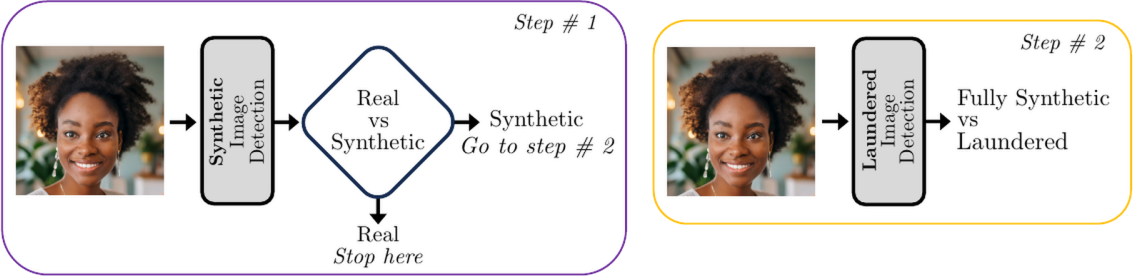
\includegraphics[width=0.95\linewidth]{Img/launder_2_stage.png}
            \caption{Visualization of the two-step architecture proposed in \cite{mandelli2024synthetic} for the laundered image classification task. The first step discriminate real images from synthetic (both fully and laundered) ones, while the second step discriminate fully synthetic images from laundered ones}
            \label{fig:launder_2_stage}
        \end{figure}
        The evaluation provided in \cite{mandelli2024synthetic} about such two-step pipeline is good: the first step reaches a good separability between real and synthetic image, while the second step reaches almost perfect results over multiple models and multiple metrics, with only minor decreases in performance when post-processing operations, like JPEG compression and resizing, are applied.

\section{Experiment}
    In this first phase of the project, we executed a preliminary experiment to asses the capability of the laundering attack (Sec. \ref{sec:laundering}) on the dataset \textit{TrueFake} provided by the \textit{MMLAB} team.

    The first phase of the experiment consisted in recovering 25 real images and, given their large size, extract 4 patches of size $1024\times1024$ from each of them, for a total of 100 real patches. Next, such patches were laundered, with a \textit{denoising} parameter of 0, using the model \textit{sd\_xl\_base\_1.0} \cite{sdxl_base_1_0}. Lastly, a total of 100 fully synthetic images, generated by \textit{Stable Diffusion XL}, were collected from the \textit{TrueFake} dataset in equal quantity from each category available.

    This small dataset was submitted to the two-step pipeline from \cite{mandelli2024synthetic}, visualized in Fig. \ref{fig:first_stage}, obtaining interesting results. The first step, as can be seen in Fig. \ref{fig:first_stage}, yielded similar results as \cite{mandelli2024synthetic}, with a good separability around threshold 0. On the other hand, the second step, in Fig. \ref{fig:second_stage}, yielded results slightly different from \cite{mandelli2024synthetic}, with the fully synthetic images average score close to 1, where \cite{mandelli2024synthetic} reported good separability at threshold 0. 

    \begin{figure}[h]
        \centering
        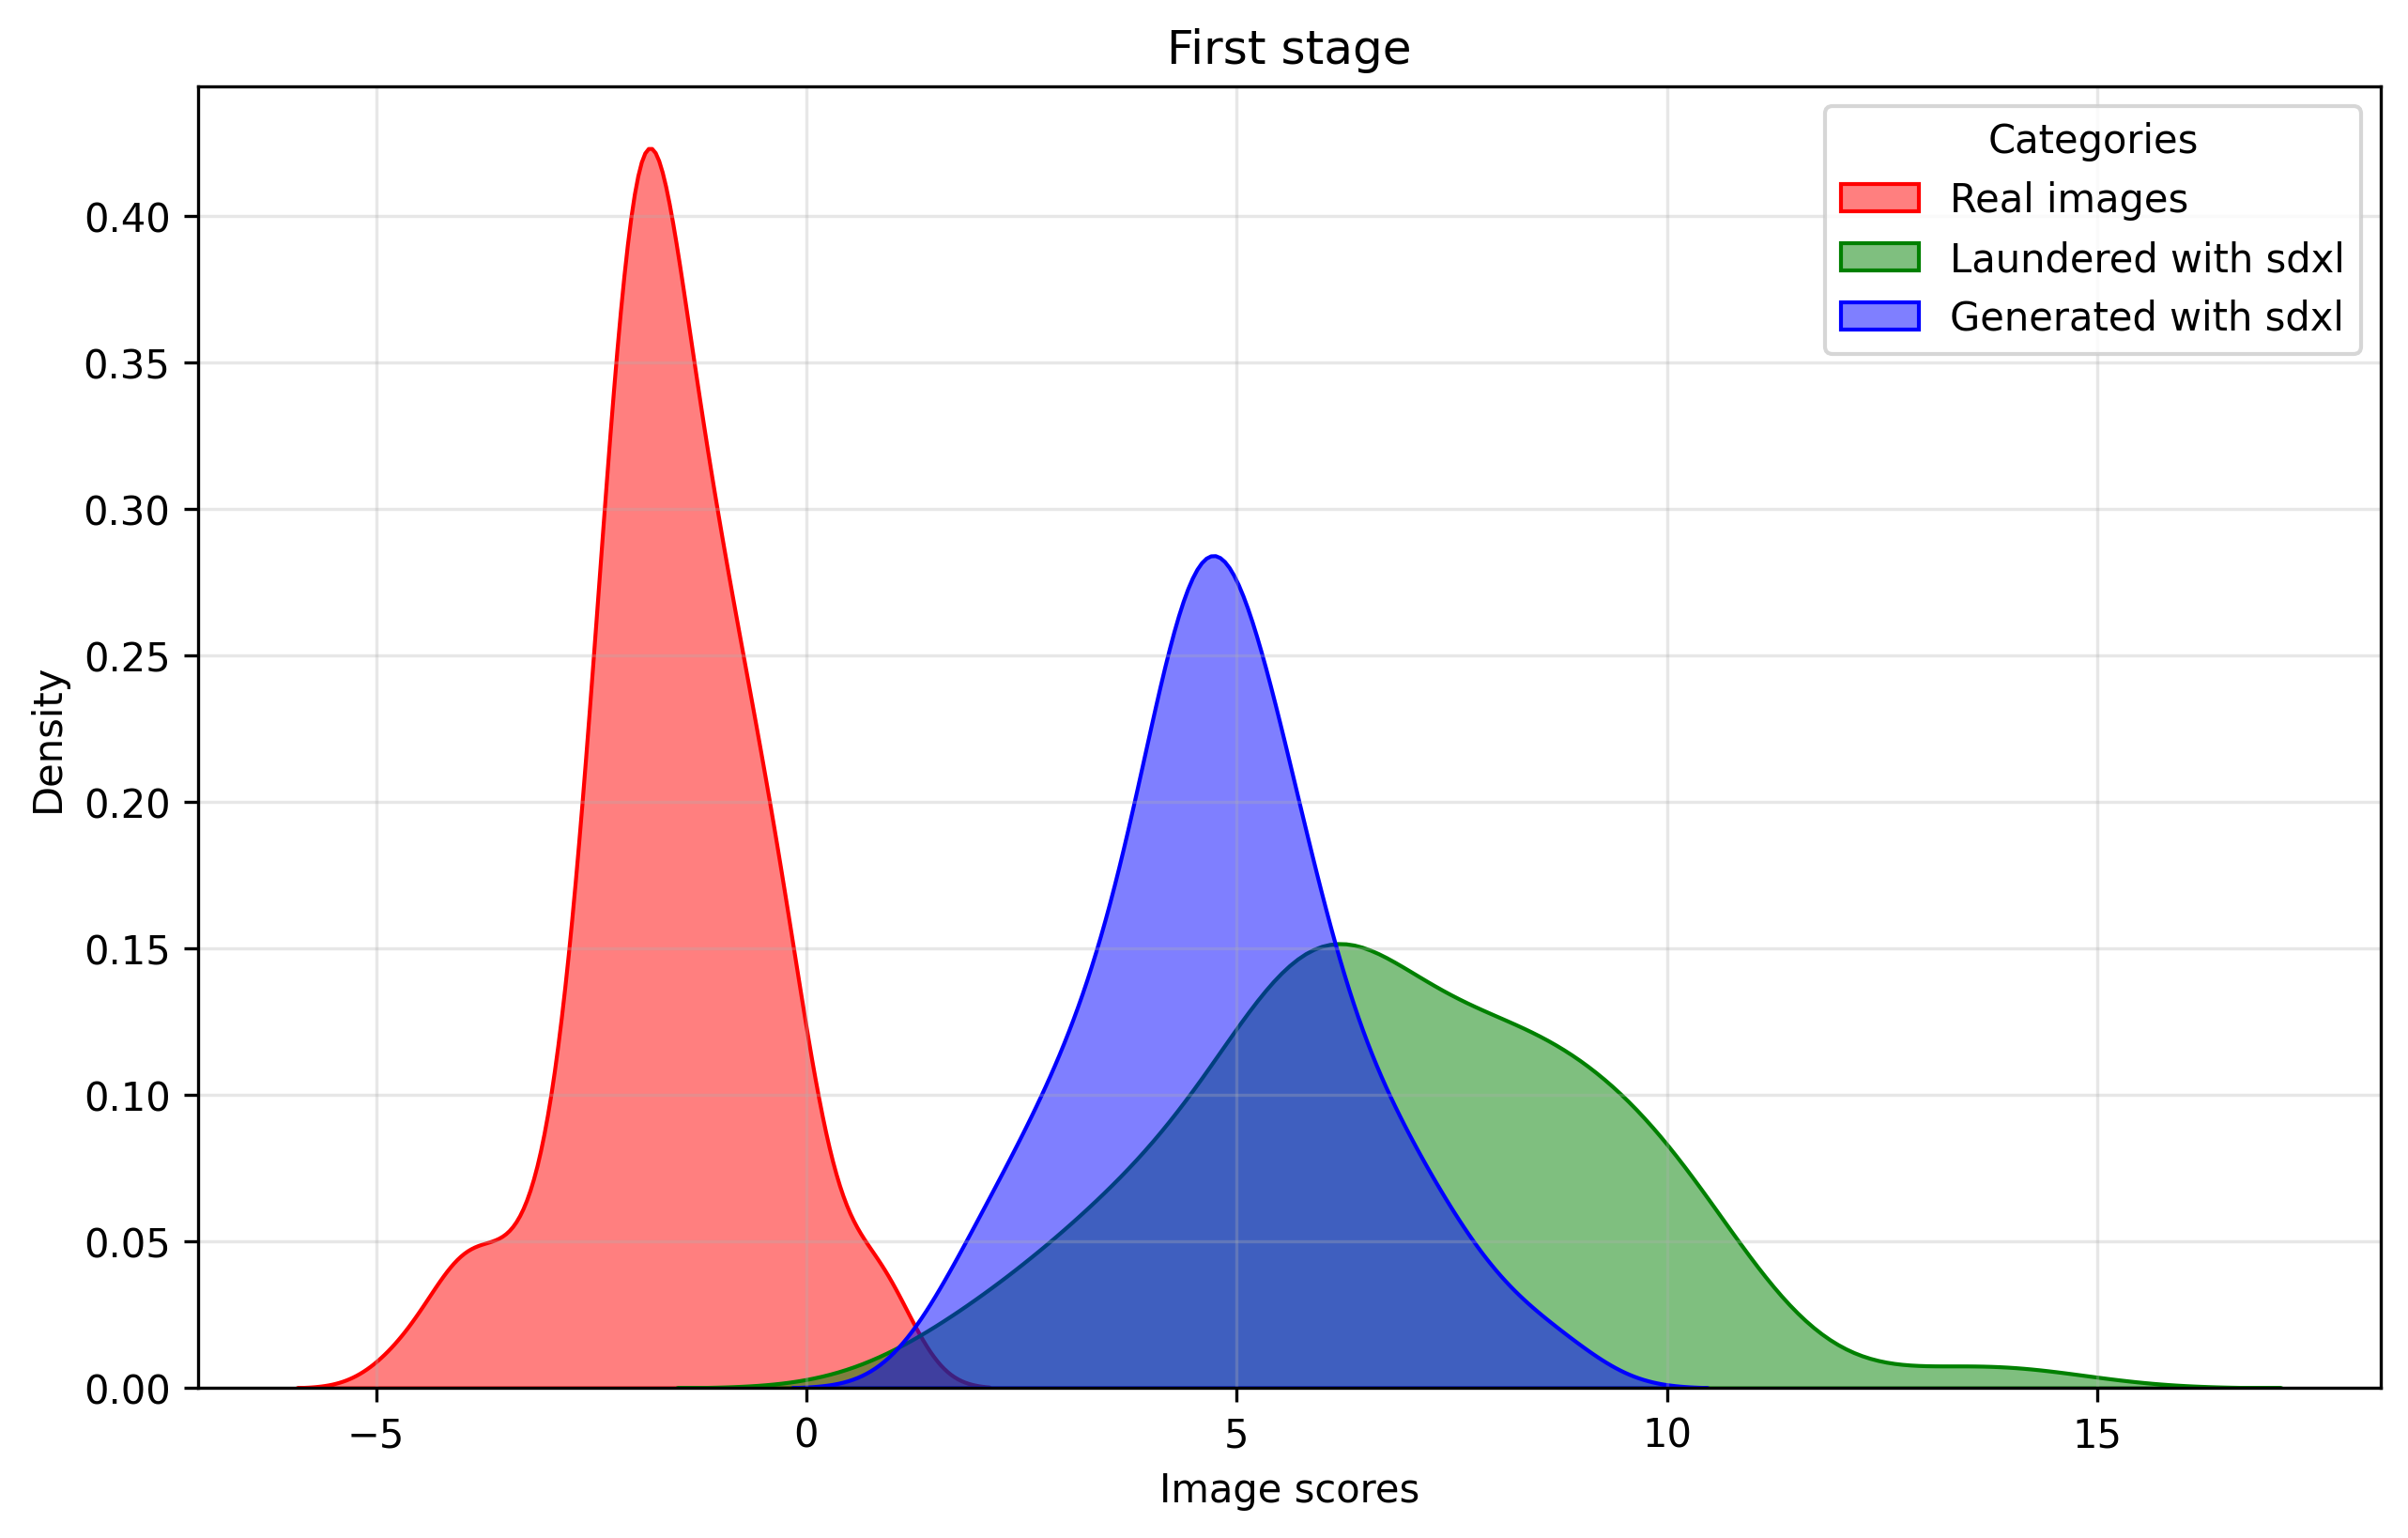
\includegraphics[width=0.95\linewidth]{Img/first_stage.png}
        \caption{Results of the first step of the pipeline from \cite{mandelli2024synthetic} using images from \textit{MMLAB TrueFake} dataset}
        \label{fig:first_stage}
    \end{figure}

    \begin{figure}[h]
        \centering
        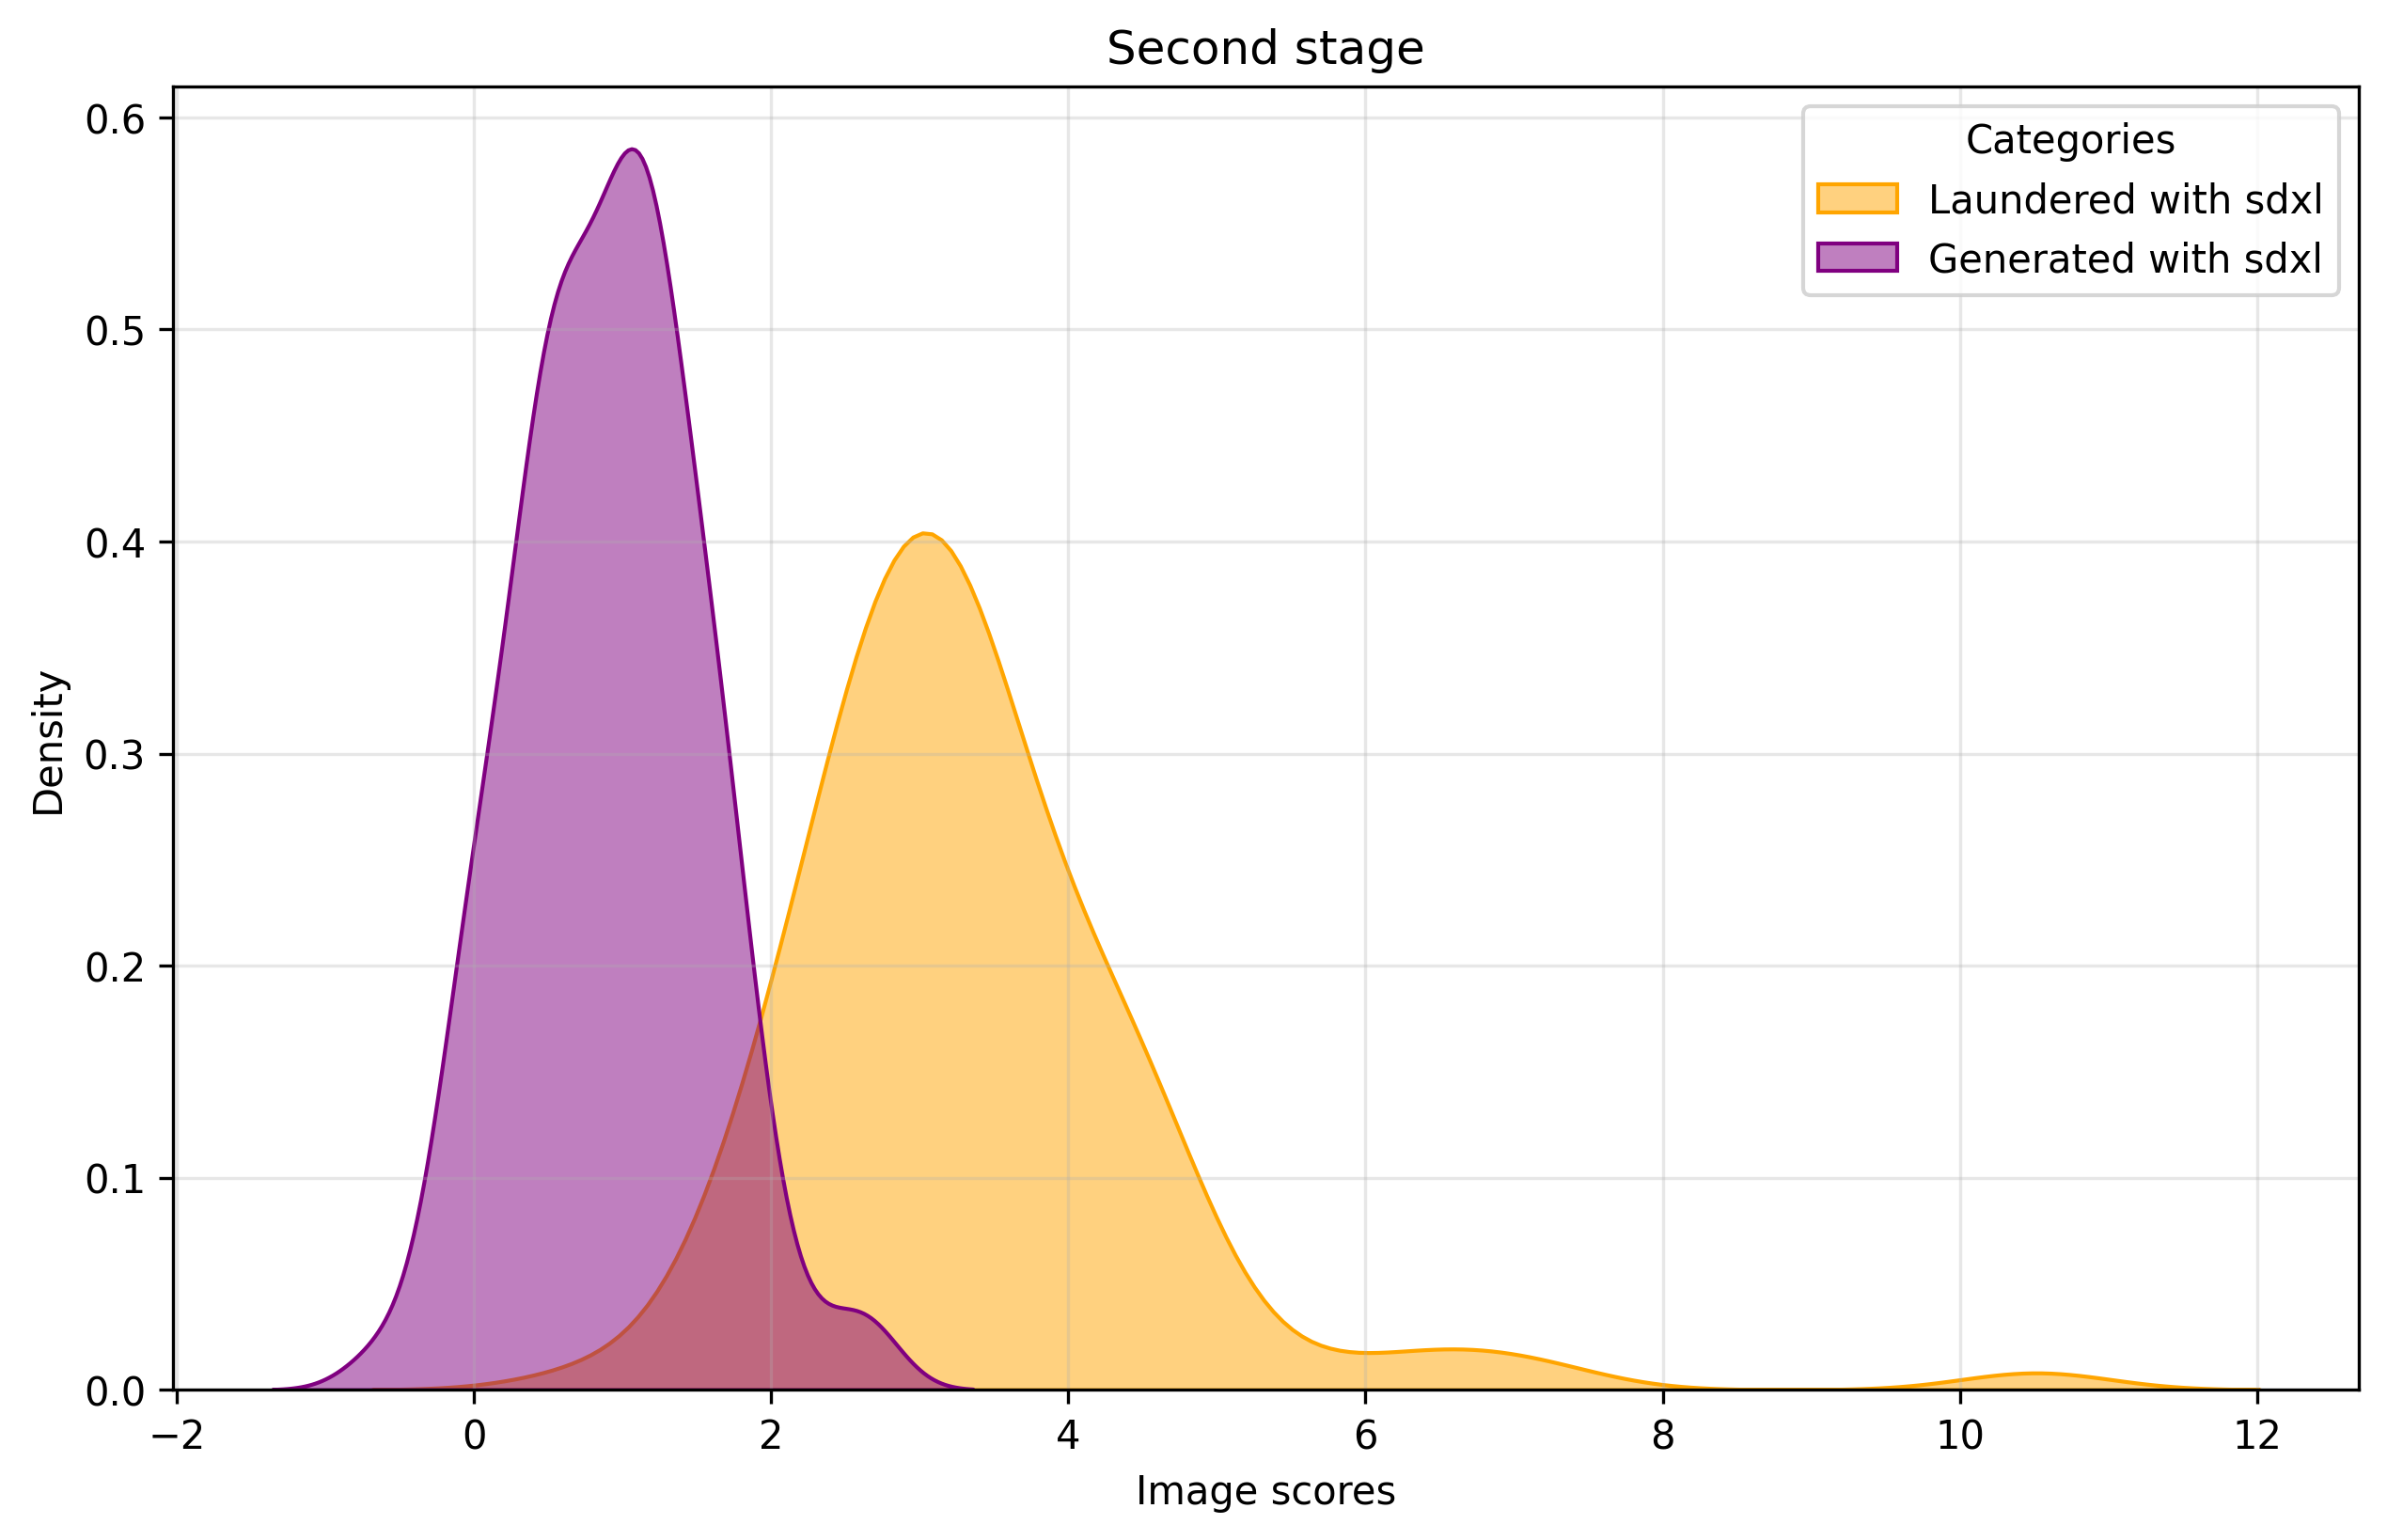
\includegraphics[width=0.95\linewidth]{Img/second_stage.png}
        \caption{Results of the second step of the pipeline from \cite{mandelli2024synthetic} using images from \textit{MMLAB TrueFake} dataset}
        \label{fig:second_stage}
    \end{figure}

\section{Conclusions}
    In this report we provided a general overview of some detection techniques and some newly implemented attack strategies. We decided to focus our future work on Diffusion Models for several reasons: 1.) they are a relatively new architecture, 2.) they can be implemented with limited hardware, 3.) for the time being there is little literature regarding them. Given the ease of use of DMs, we assume that more and more people will use them, hence the necessity to provide solid performance evaluations of current SoTA detectors and to assess the capabilities of the attacks based on these architectures.

    The next phases of our work will focus on continuing the experiments with the \textit{MMLAB} dataset, assessing the performance of the described approaches and the capabilities of the proposed attacks.

\bibliographystyle{IEEEtran} % Stile delle referenze (es. IEEE)
\bibliography{references}    % Nome del file .bib (senza estensione)

\end{document}